%%%%%%%%%%%%%%%%%%%%%%%%%%%%%%%%%%%%%%%%%%%%%%%%%%%%%%%%%%%%%%%%%%%%%%
% Slides
%%%%%%%%%%%%%%%%%%%%%%%%%%%%%%%%%%%%%%%%%%%%%%%%%%%%%%%%%%%%%%%%%%%%%%

\begin{frame}
\titlepage
\end{frame}

\begin{frame}{Overview}
  \tableofcontents
\end{frame}

\section{Revisão Teórica}

\begin{frame}{BIG DATA ?}
    \begin{itemize}
    \item A sociedade está lidando com uma quantidade de dados cada vez maior.
    \item Os dados precisam de tratamentos;
    \item Os dados geram informações importantes.
    \item A informação é o diferencial
    \item Massa de dados de grande volume, velocidade e variedade.
    \end{itemize}
\end{frame}

\begin{frame}{Relacional x NoSQL}
    \begin{itemize}
    \item O modelo relacional representa o banco de dados como uma coleção de relações;
    \item Validação, verificações e garantias de integridade, controle de concorrências...
    \item Problemas causados pelo layout rígido.
    \item PostgreSQL, MySQL, Oracle, MS SQL, DB2
    \end{itemize}
\end{frame}

\begin{frame}{Relacional x NoSQL}
	\begin{figure}[!htbp]
		\begin{center}
			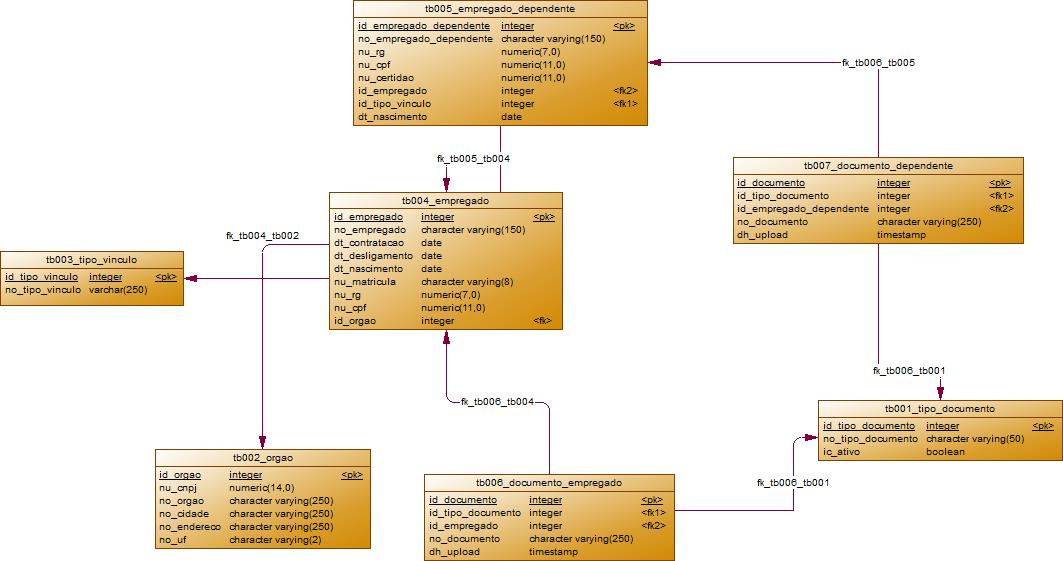
\includegraphics[width=0.8\textwidth]{modelo_relacional}
		\end{center}
		\caption{Modelo Relacional }
		\label{fig:modelorelacional}
	\end{figure}
\end{frame}

\begin{frame}{Relacional x NoSQL}
    \begin{itemize}
    \item Armazenamento de dados de forma não relacional;
    \item Schema free;
    \item Chave-Valor / Orientados a Documentos / Orientados a Colunas / Baseados em Grafos;
    \item Google, Amazon, Facebook...
    \item MongoDB, Cassandra, NEO4j, Redis
    \end{itemize}
\end{frame}

\begin{frame}{Relacional x NoSQL}
	\begin{figure}[!htbp]
		\begin{center}
			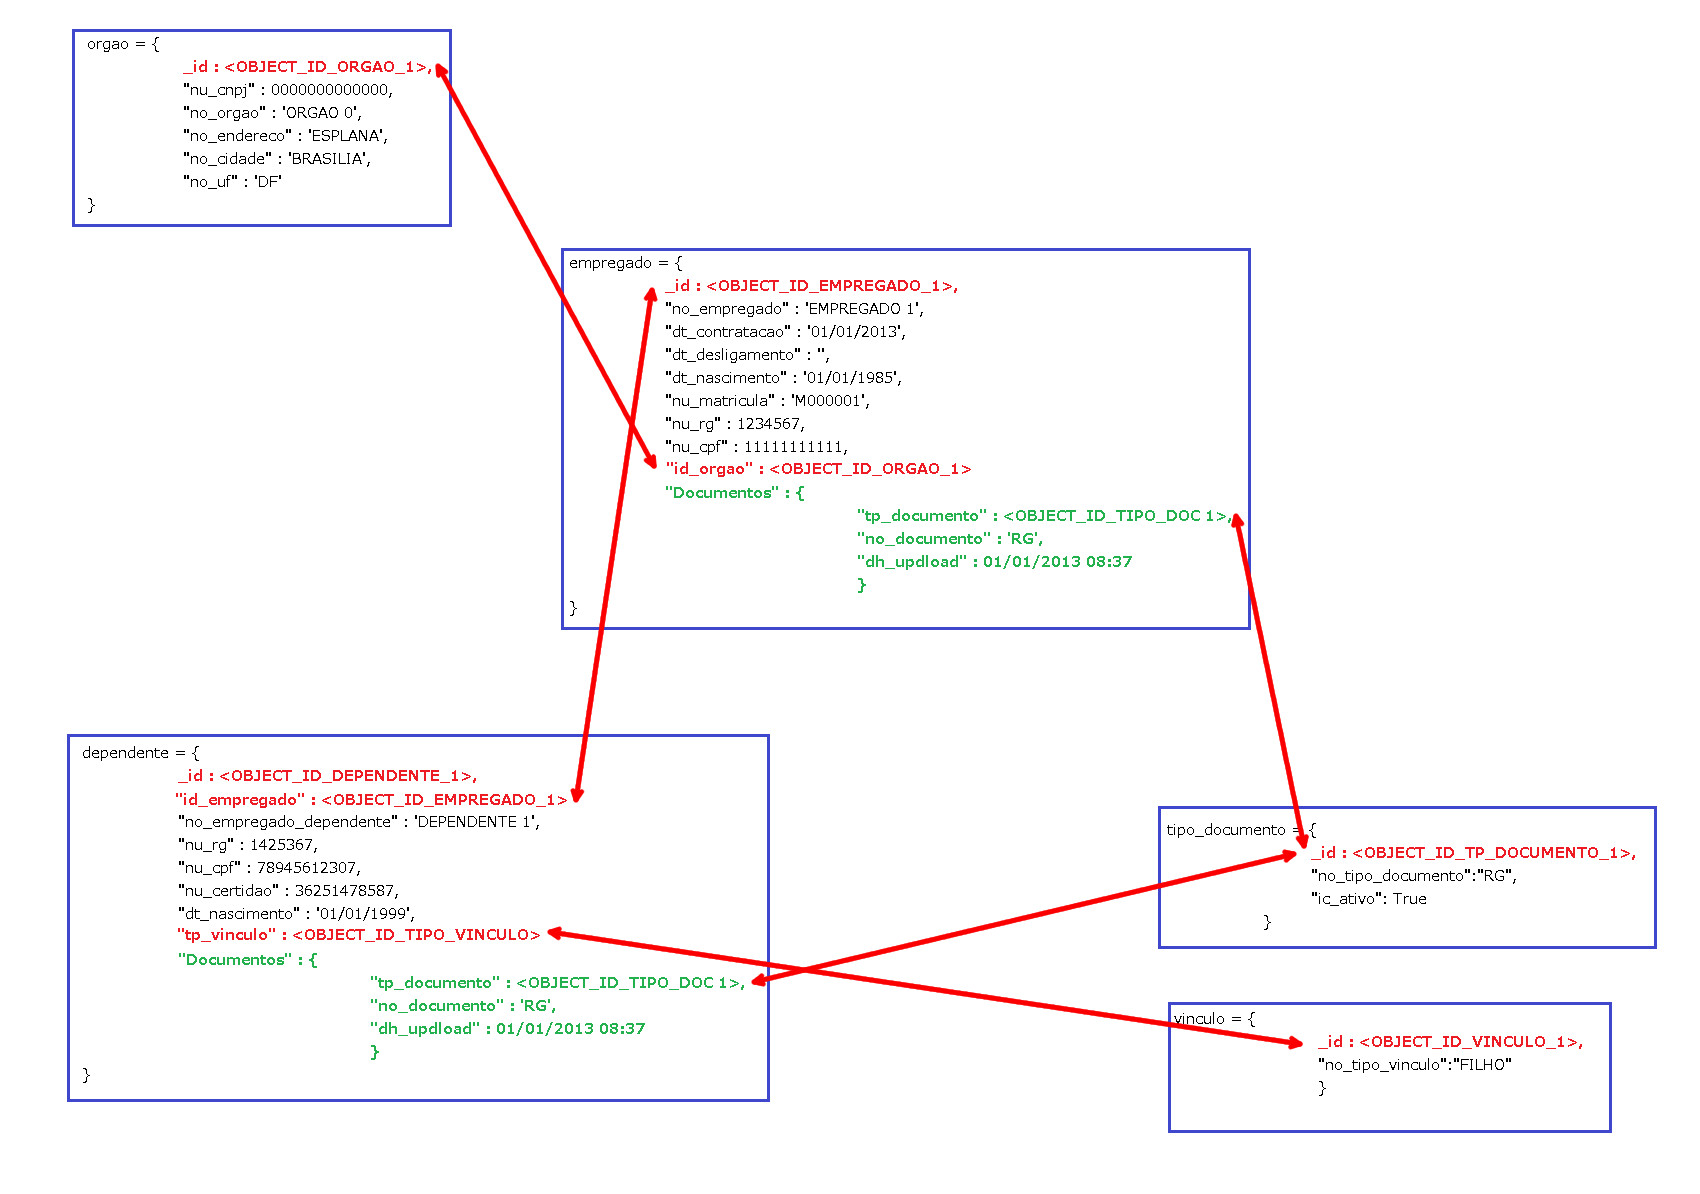
\includegraphics[width=0.9\textwidth]{modelo_orientado_documentos}
		\end{center}
		\caption{ Modelagem orientada a documentos implementada no protótipo.}
		\label{fig:modeloorientadodocumentos}
	\end{figure}
\end{frame}

\section{O Projeto}

\begin{frame}{O Projeto}
    \begin{itemize}
	\item Grande número de pastas funcionais físicas geram custos para manter a qualidade dos arquivos permanentes;
	\item Digitalização das pastas funcionais;
    \end{itemize}
\end{frame}

\begin{frame}{O Projeto}
    \begin{itemize}
	\item AFD - Criação de um dossiê, em mídia digital;
	\item Fonte Primária de informações cadastrais do Servidor Público Civil Federal. \textit{citar site do SIGEPE}
    \end{itemize}
\end{frame}

\begin{frame}{Problema}
    \begin{itemize}
           \item Determinar se um banco de dados NoSQL é indicado para um caso como o citado e se temos um tipo de banco mais adequado.
    \end{itemize}
\end{frame}


\begin{frame}{Hipótese}
    \begin{itemize}
           \item Podemos melhorar a performance nas consultas e armazenamento, porém o grau de consistência e confiabilidade necessários devem ser medidos e implementados na aplicação.
    \end{itemize}
\end{frame}


\begin{frame}{Motivação}
    \begin{itemize}
    \item Tema relativamente novo;
    \item Caso Real;
    \item Mercado -> Academia;
    \item Novas Tecnologias;
    \end{itemize}
\end{frame}


\begin{frame}{Objetivo Geral}
    \begin{itemize}
    \item Comparar os modelos relacional e não relacional (Orientada a Documento) de armazenamento  para o contexto do Assentamento Digital Funcional (AFD).
    \end{itemize}
\end{frame}


\begin{frame}{Objetivos Específicos}
    \begin{itemize}
    \item Compreender, abstrair e modelar os conceitos e operações do AFD;
    \item Modelar os conceitos do AFD utilizando a estratégia relacional;
    \item Modelar os conceitos do AFD utilizando a estratégia orientada a documentos;
    \item Implementar os modelos em SGBDs relacionais e orientados a documentos;
%    \item Implementar uma arquitetura SOA para realizar as operações do AFD, utilizando os dois bancos para a persistência;
%   \item Projetar, implementar e realizar testes de desempenho que nos permitam tirar conclusões sobre quais dos modelos são mais %propícios para o armazenamento dos dados do AFD.
    \end{itemize}
\end{frame}

\begin{frame}{Objetivos Específicos}
    \begin{itemize}
    \item Implementar uma arquitetura SOA para realizar as operações do AFD, utilizando os dois bancos para a persistência;
   \item Projetar, implementar e realizar testes de desempenho que nos permitam tirar conclusões sobre quais dos modelos são mais propícios para o armazenamento dos dados do AFD.
    \end{itemize}
\end{frame}

\begin{frame}{Resultados Esperados}
    \begin{itemize}
    \item Obter informações o bastante para escolher o banco de dados mais indicado para esse caso e semelhantes.
    \end{itemize}
\end{frame}


\begin{frame}{Metodologia}
    \begin{itemize}
    \item Entender o problema;
    \item Estudar as soluções;
    \item Testar as soluções;
    \end{itemize}
\end{frame}

\section{Cronograma}

\newenvironment{changemargin}[2]{%
  \begin{list}{}{%
    \setlength{\topsep}{0pt}%
    \setlength{\leftmargin}{#1}%
    \setlength{\rightmargin}{#2}%
    \setlength{\listparindent}{\parindent}%
    \setlength{\itemindent}{\parindent}%
    \setlength{\parsep}{\parskip}%
  }%
  \item[]}{\end{list}}


\begin{frame}
\begin{changemargin}{-1cm}{-1cm} 
\begin{table}[h]
	\begin{center}
	\begin{tabular}{ p{4cm}lcccccc}
		\hline
			\textbf{Tarefas} & \textbf{JUL} & \textbf{AGO} & \textbf{SET} & \textbf{OUT} & \textbf{NOV} & \textbf{DEZ}\\
		\hline
			Escrita da Monografia & x & x & x & x & x & x\\
			Compreender AFD & x & x &  &  &  & \\
			Modelagem Relacional &  &  & x &  &  & \\
			Modelagem Orientada a  Documentos &  &  & x & x &  & \\
			Implem. Mod. de Dados &  &  & x & x &  & \\
			Arquitetura SOA &  & x & x & x & x & \\
			Projeto e Implem. Testes &  &  & x & x & x & \\
			Execução dos Testes &  &  &  &  & x & x\\
		\hline
	\end {tabular}
	\end{center}
\end{table}
\end{changemargin}
\end{frame}

\section{Referências}

\begin{frame}{Bibliografia I}
\begin{itemize}

\item E. Hewitt. Cassandra: The Definitive Guide. Definitive Guide Series. O'Reilly Media,
2010.

\item S. Tiwari. Professional NoSQL. Wrox Programmer to Programmer. Wiley, 2011.

\item Mongodb oficial site. \url{http://www.mongodb.org/}

\end{itemize}
\end{frame}

\begin{frame}{Bibliografia II}
\begin{itemize}

\item R. Hecht and S. Jablonski. Nosql evaluation: A use case oriented survey. In Cloud
and Service Computing (CSC), 2011 International Conference on, pages 336 - 341,
dec. 2011.
\end{itemize}
\end{frame}

\begin{frame}{Bibliografia III}
\begin{itemize}

\item Vinayak R. Borkar, Michael J. Carey, and Chen Li. Big data platforms: What's
next? XRDS, September 2012.

\item Ricardo W. Brito. Banco de dados nosql x sgbds relacionais: Análise comparativa.
2010.
\end{itemize}
\end{frame}

\appendix

\begin{frame}
  \frametitle{Obrigado pela atenção!}
  \begin{center}
    {\Huge Obrigado!}
  \end{center}
\end{frame}
